\documentclass[11pt]{article}
\usepackage{color} %used for font color
\usepackage{amssymb} %maths
\usepackage{amsmath} %maths
\usepackage{epsfig}
\usepackage{amsmath, bm}
\usepackage{enumitem}
\topmargin-.5in
\textwidth6.6in
\textheight9in
\oddsidemargin0in
\usepackage{graphicx}
\usepackage{subfig}
\def\ds{\displaystyle}
\def\d{\partial}
\def\bH{{\bf H}}
\def\bM{{\bf M}}
\def\bB{{\bf B}}
\def\bm{{\bf m}}
\def\bS{{\bf S}}
\def\hQ{{\Phi}}
\def\ve{{\varepsilon}}
%\def\fs{\scriptsize}
\def\fs{\footnotesize}
\def\reals{\mathbb{R}}
\def\complex{\mathbb{C}}
\def\scriptO{{{\it O}\kern -.42em {\it `}\kern + .20em}}

\begin{document}

\centerline{\large \bf Math 540: Project 4}

\bigskip
\noindent
$$\mathbf{Tilekbek\,\,\,\, Zhoroev}$$
\begin{enumerate}
\item Consider the height-weight model $$ Y_i = \theta_0 +\theta_1(x_i/12)+ \theta_2(x_i/12)^2 +\varepsilon_i$$ with the data compiled in Table \ref{tab1}. Using the parameter and covariance matrix estimates $$\pmb{\theta} = \begin{bmatrix} 261.88\\ -88.18\\ 11.96\end{bmatrix}, \quad \pmb{V} = \begin{bmatrix} 634.88 & -235.04& 21.66\\  -235.04& 87.09 & -8.03\\ 21.66& -8.03& 0.74\end{bmatrix} $$ compute and plot $2\sigma$ and frequentist prediction intervals, along with the data, for heights ranging from 58 to 72 inches. Repeat this for the extrapolatory regime of 50 to 80 inches and discuss your results.

\begin{table}[ht!]
\centering
\begin{tabular}{|l|l|l|l|l|l|l|l|l|l|l|l|l|l|l|l|}
\hline
\multicolumn{1}{|c|}{\begin{tabular}[c]{@{}c@{}}Height\\ (in)\end{tabular}} & 58  & 59  & 60  & 61  & 62  & 63  & 64  & 65  & 66  & 67  & 68  & 69  & 70  & 71  & 72  \\ \hline
\begin{tabular}[c]{@{}c@{}}Weight\\ (lbs)\end{tabular}                      & 115 & 117 & 120 & 123 & 126 & 129 & 132 & 135 & 139 & 142 & 146 & 150 & 154 & 159 & 164 \\ \hline
\end{tabular}
\caption{Height-weight data}
\label{tab1}
\end{table}


{\em Solution} The design matrix in this case $$\mathbf{X}=\begin{bmatrix} 1 & x_1/12 & (x_1/12)^2\\ 1 & x_2/12 & (x_2/12)^2\\
\vdots & \vdots & \vdots\\
1 & x_n/12 & (x_n/12)^2
\end{bmatrix}$$ where $x_i$ given data points for $i=1,2,3,...., n =15.$ Next, we can find the relative residuals and, by using them we can obtain the variance, $\sigma^2$ and covariance matrix, $\mathbf{}{V}.$ Since $\mathbb{E}[\mathbf{Y}] = \mathbf{X}\pmb{\theta_0}$  and cov$[\mathbf{Y}] = \mathbf{XVX}^\top + \mathbf{}{V}_{obs},$ where $\pmb{V}_{obs} = \sigma^2 \mathbf{I}_{n}$ the $\pm 2\sigma_{\pmb{Y}}$ interval  becomes 
$$ \bigg[\mathbf{X}_i \pmb{\theta}_0 \pm 2\sqrt{(\mbox{cov}[\mathbf{Y}])_{ii}} \bigg]$$ where $\mathbf{X}_i$ is the $i'$th row of the design matrix. The $(1-\alpha)\times 100\%$ frequentist prediction interval  at $x_{*}$ is $$\Bigg[\hat Y_{x_{*}} \pm t_{n-p, 1-\alpha/2}\hat\sigma  \sqrt{1+x_*(\mathbf{X^\top X})^{-1}x_{*}^\top} \Bigg].$$  

Employing these formulas, we obtain the $\pm2\sigma_\mathbf{Y}$ and frequentist $95\%$ prediction interval, in Figure \ref{fig1}(a). From the graph, we observe that both the intervals are the same and all the given data points are inside of the intervals. Next, we redo the same analysis in the interval [50, 80] and the  $\pm2\sigma_\mathbf{Y}$  and frequentist $95\%$ prediction interval, in Figure \ref{fig1}(b). Here we observe that the prediction interval for the extrapolation domain is wider than the calibration domain. 

\begin{figure*}[!htb]
   \subfloat[]{%
      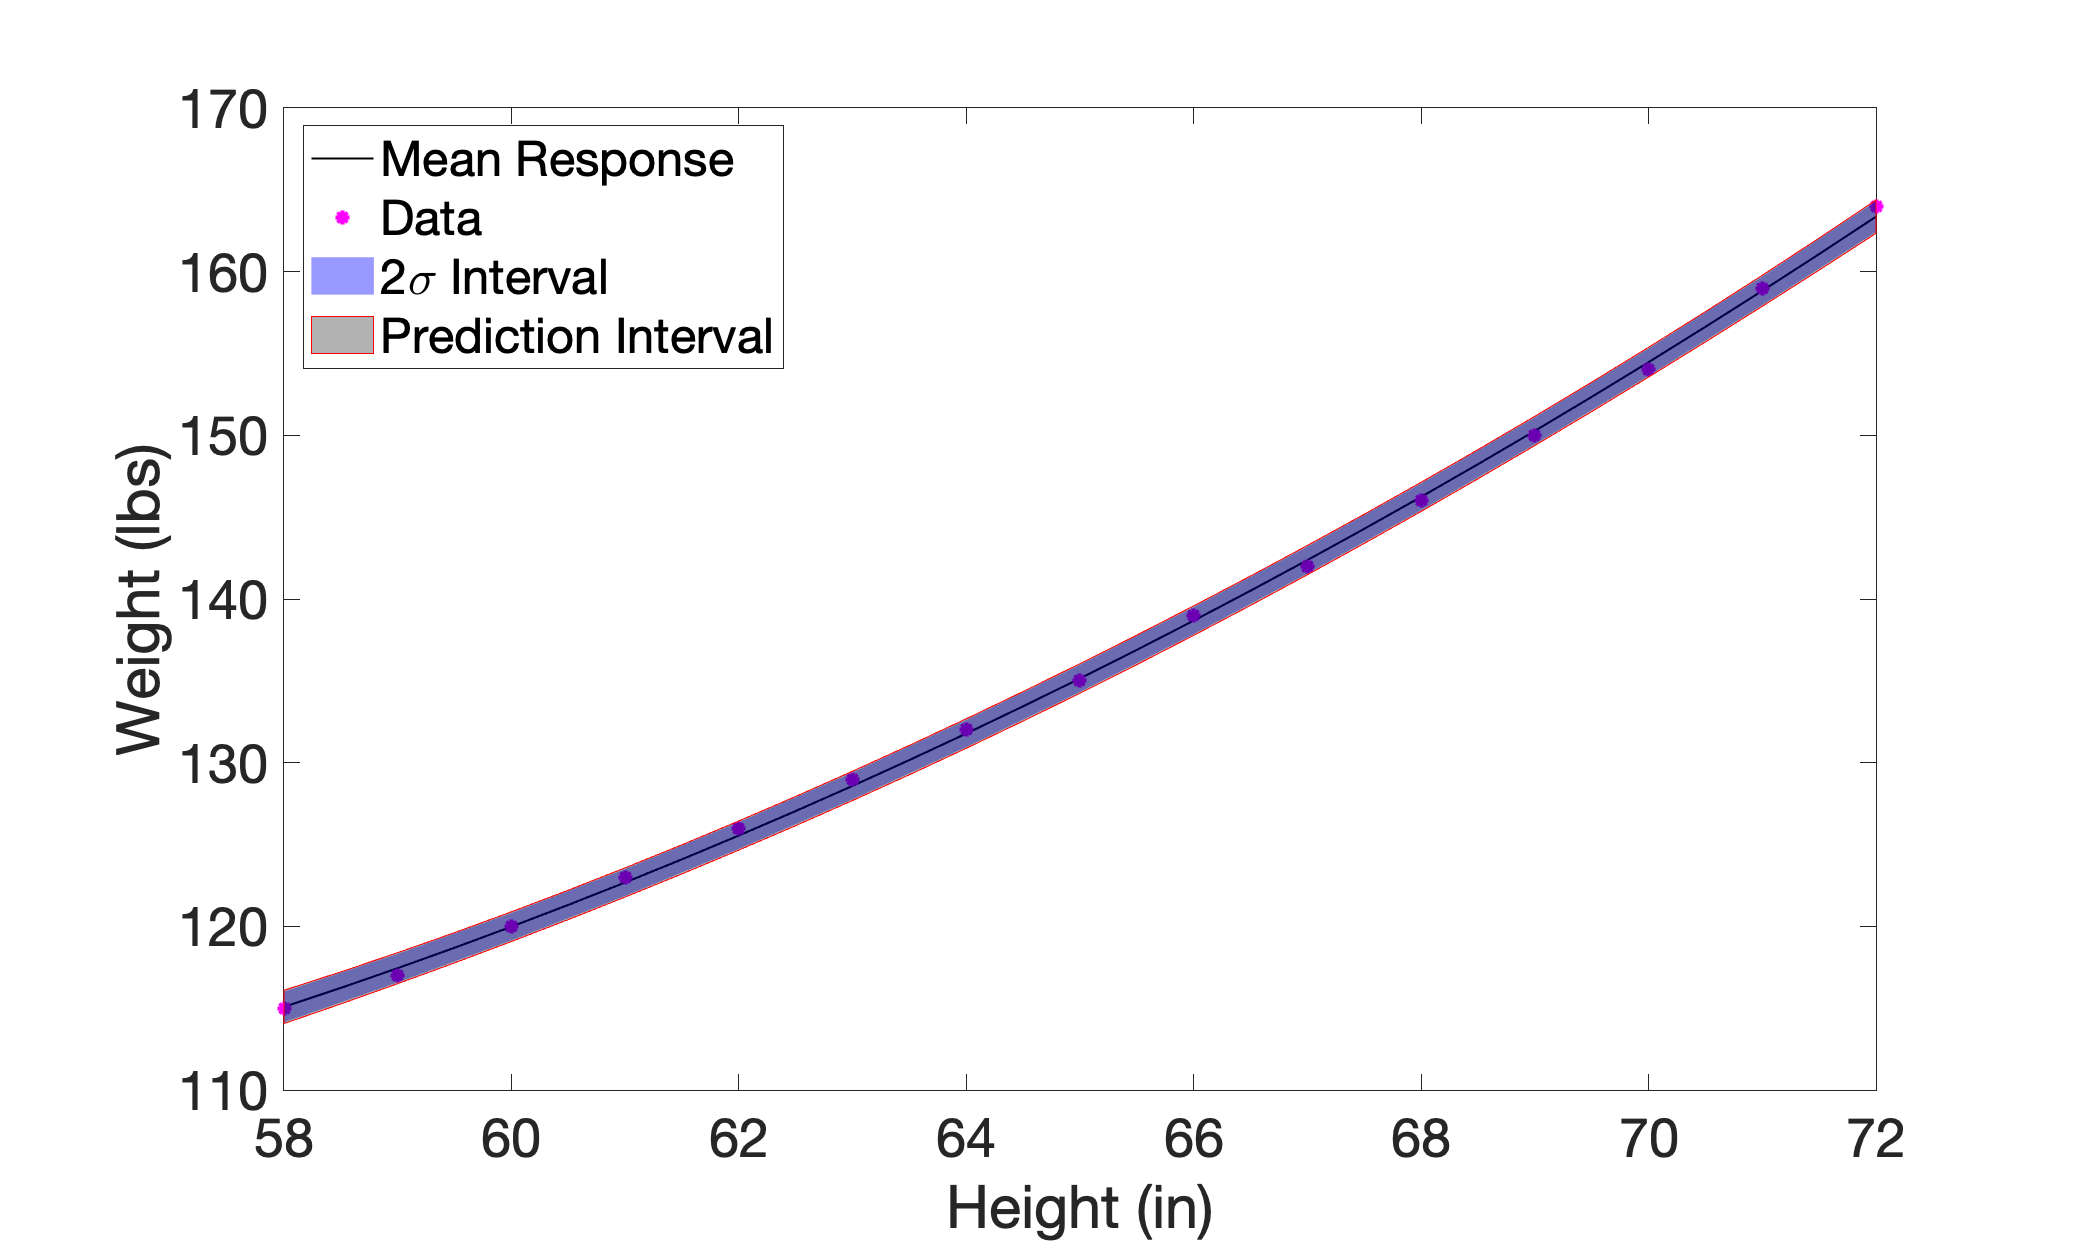
\includegraphics[ width=.5\linewidth]{Figures/1a.eps}}
   \subfloat[]{%
      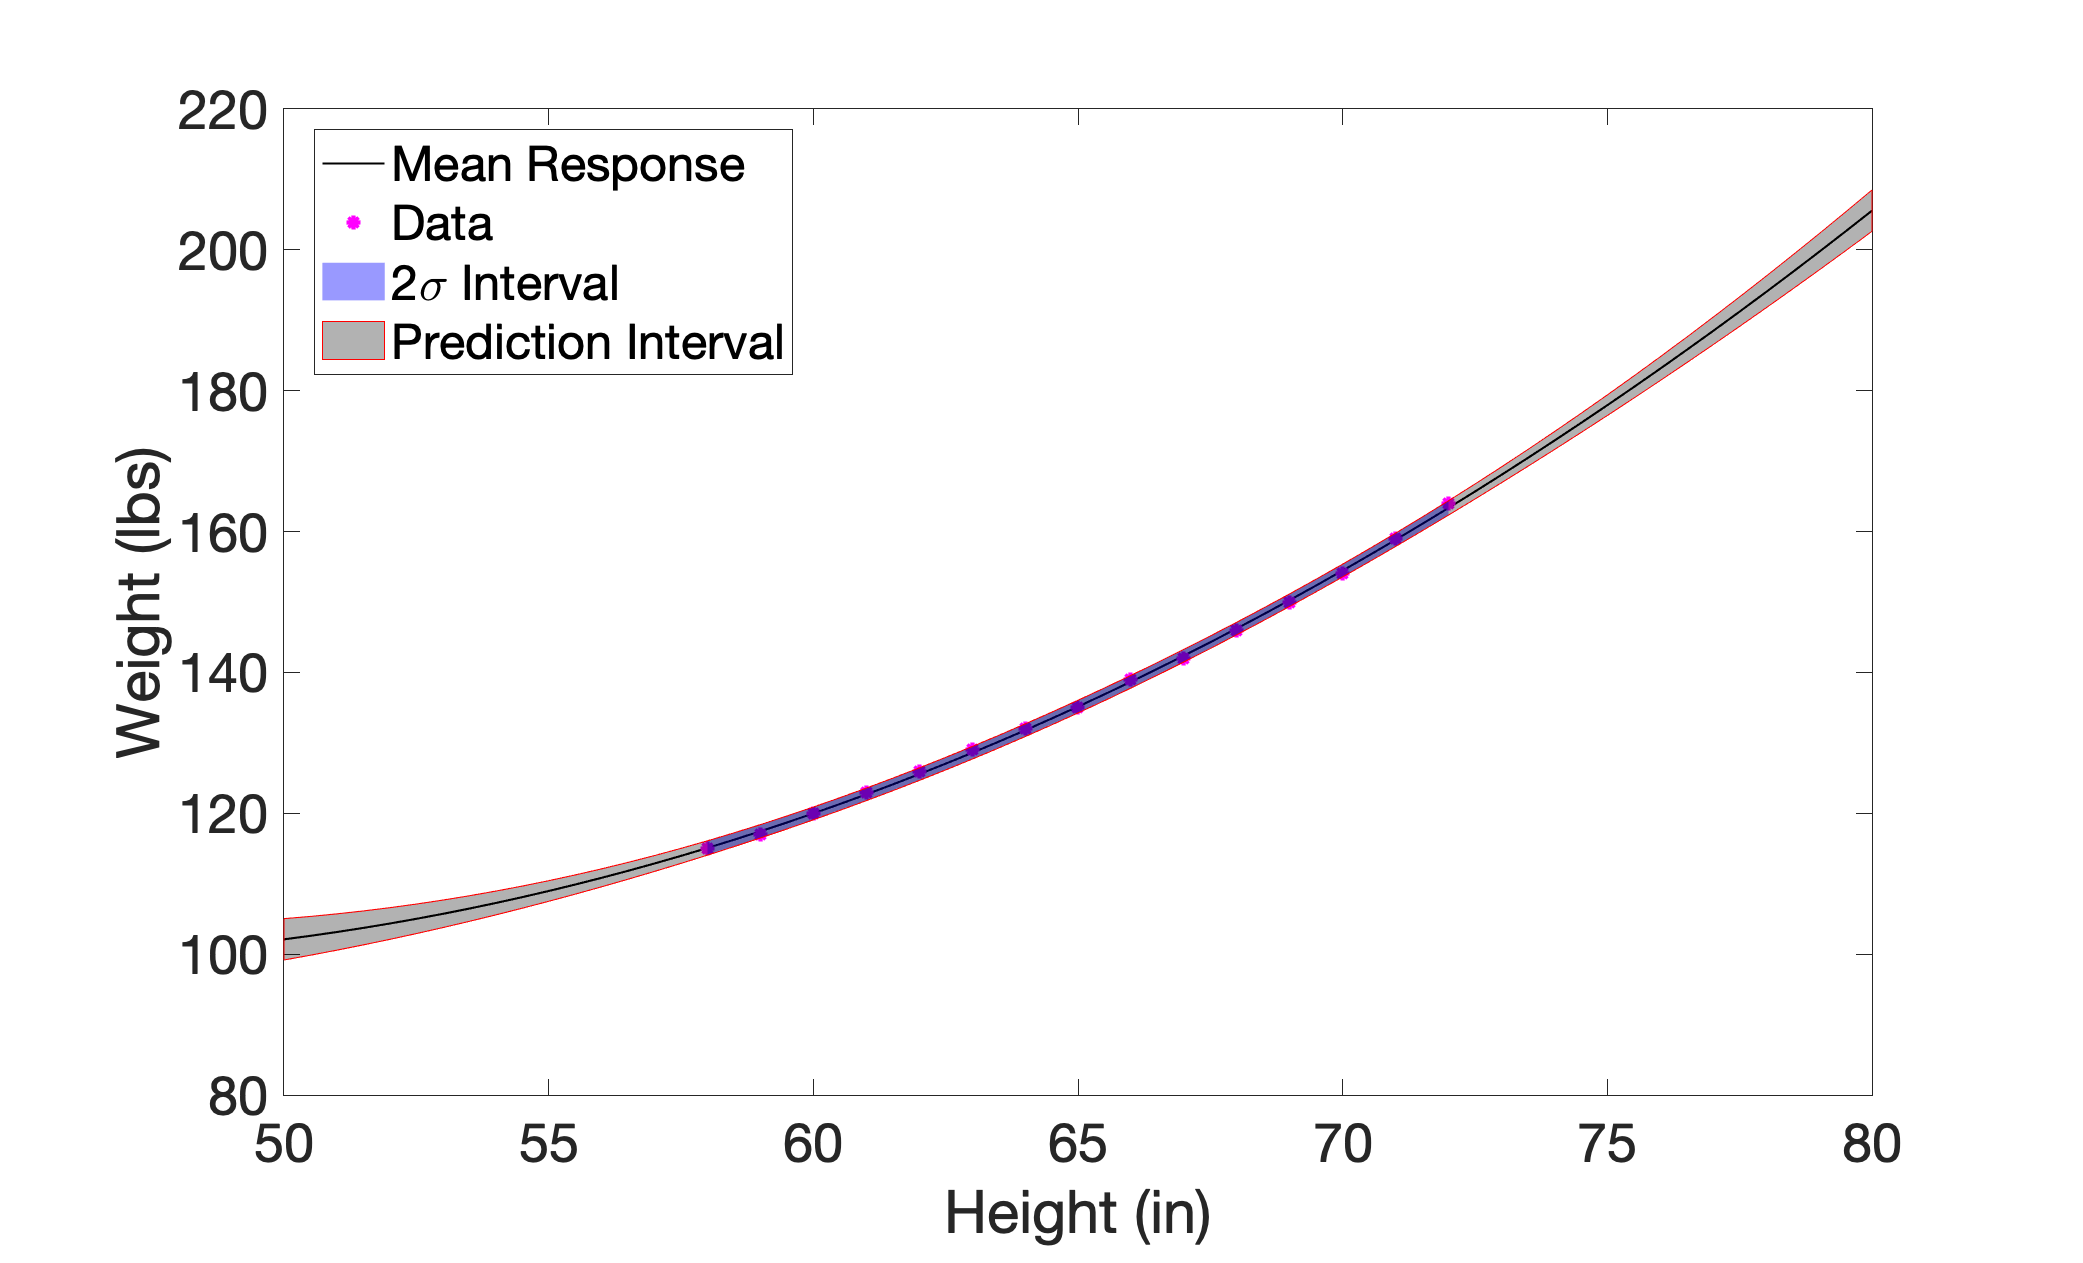
\includegraphics[ width=.5\linewidth]{Figures/1b.eps}}\\
\caption{Data, $2\sigma_{\mathbf{Y}}$ and prediction intervals for (a) calibration domain [58, 72] and (b)
extrapolation domain [50, 80]}
\label{fig1}
\end{figure*}

\item 
Consider the steady state heat model
\begin{align*}
    \frac{d^2\, u_{s}(x)}{d x^2}&=\frac{2(a+b)h}{kab}[u_{s}(x)-u_{amb}],  \quad 0<x<L\\
   \frac{d\,u_{s}}{dx}(0)& = \frac{\Phi}{k} \\
   \frac{d \,u_{s}}{d x}(L)&= \frac{h}{k} [u_{amb} - u_{s}(L)] .
\end{align*} detailed in Example 3.9 and illustrated in Example 12.17 in the context of Bayesian model calibration. Here we employ a subset of the data from Table \ref{tab2} to construct prediction intervals that extrapolate beyond the calibration domain. Employ the DRAM  to construct densities for $\Phi$, $h$, and $\varepsilon$ using the data compiled in Table \ref{tab3}. You can use the thermal conductivity value k = 2.37 for aluminum. By sampling from the densities, construct credible and prediction intervals for $x\in [10, 66]$ and plot with the complete data set from Table \ref{tab2}. 



\begin{table}[!htb]
\centering
\scriptsize
\begin{tabular}{|c|l|l|l|l|l|l|l|l|l|l|l|l|l|l|l|}
\hline
x (cm)  & 10    & 14    & 18    & 22    & 26    & 30    & 34    & 38    & 42    & 46    & 50    & 54    & 58    & 62    & 66    \\ \hline
Temp ($^{\circ}$C) & 96.14 & 80.12 & 67.66 & 57.96 & 50.90 & 44.84& 39.75 & 36.16 & 33.31 & 31.15 & 29.28& 27.88 & 27.18 & 26.40 & 25.86 \\ \hline
\end{tabular}
\caption{Steady-state  temperatures measured at locations x for an aluminum  rod.}
\label{tab2}
\end{table}
\begin{table}[!htb]
\centering
\begin{tabular}{|l|l|l|l|l|l|l|l|l|l|}
\hline
x (cm)   & 22    & 26    & 30    & 34    & 38    & 42    & 46    & 50    & 54    \\ \hline
Temp($^{\circ}$C) & 57.96 & 50.90 & 44.84 & 39.75 & 36.16 & 33.31 & 31.15 & 29.28 & 27.88 \\ \hline
\end{tabular}
\caption{Steady-state temperatures at locations x for an aluminum rod.}
\label{tab3}
\end{table}

{\em Solution.} Since the parameter estimations and covariance matrices are given in Example 12.17, we would use these results to start the DRAM algorithm. After obtaining all the chains, we observe that all the chains have converged. Moreover, the covariance of the chain is  $$\mathbf{V} = \begin{bmatrix}    1.3538 \times 10^{-1}  & -1.0206 \times 10^{-5} \\ -1.0206 \times 10^{-5} &  7.9377 \times 10^{-10}\end{bmatrix}$$ and the variance $\sigma^2 =0.0461.$ Then using chains and $\mathbf{kde.m}$ we construct densities for $\Phi, h,$ and $\varepsilon$ given in Figure \ref{fig2}.

\begin{figure*}[!htb]
\centering
   \subfloat[]{%
      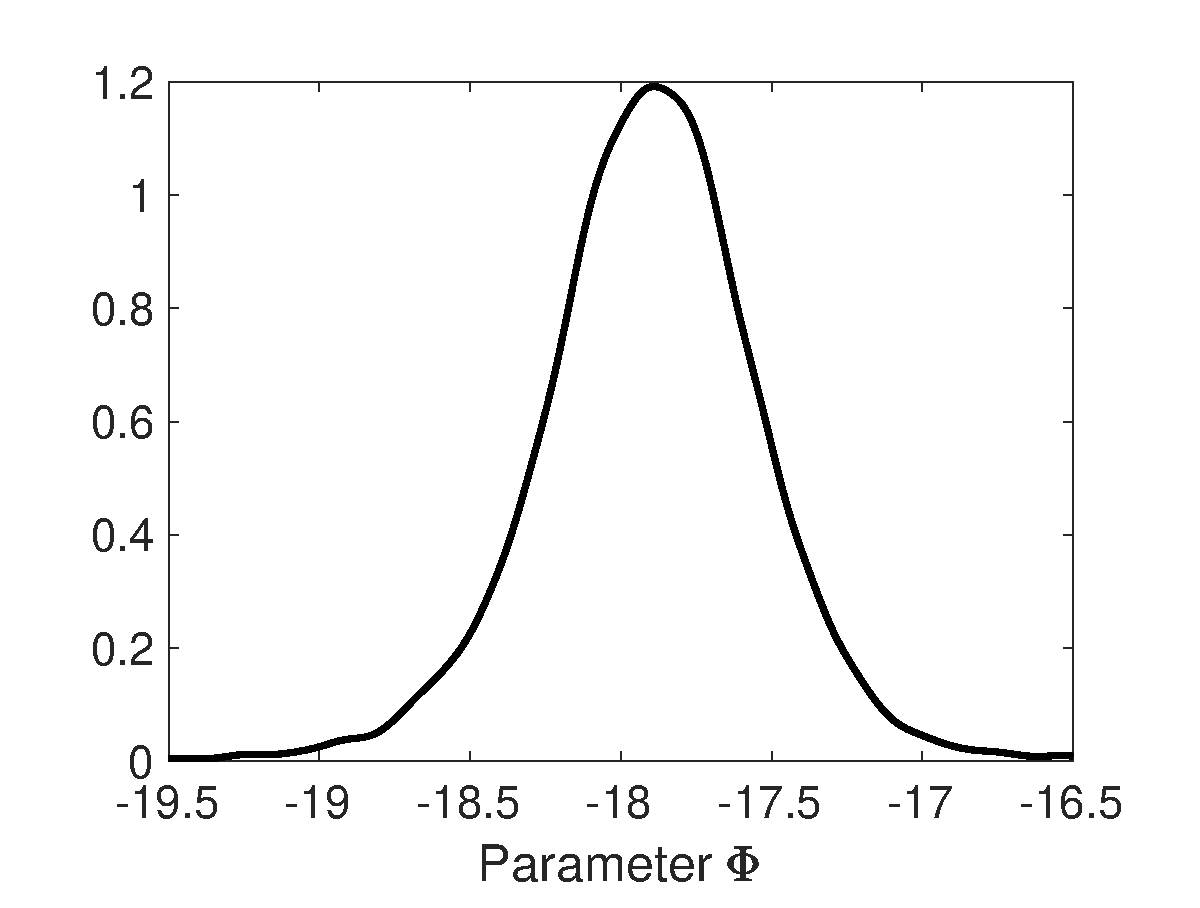
\includegraphics[ width=.5\linewidth]{Figures/2c.eps}}
   \subfloat[]{%
      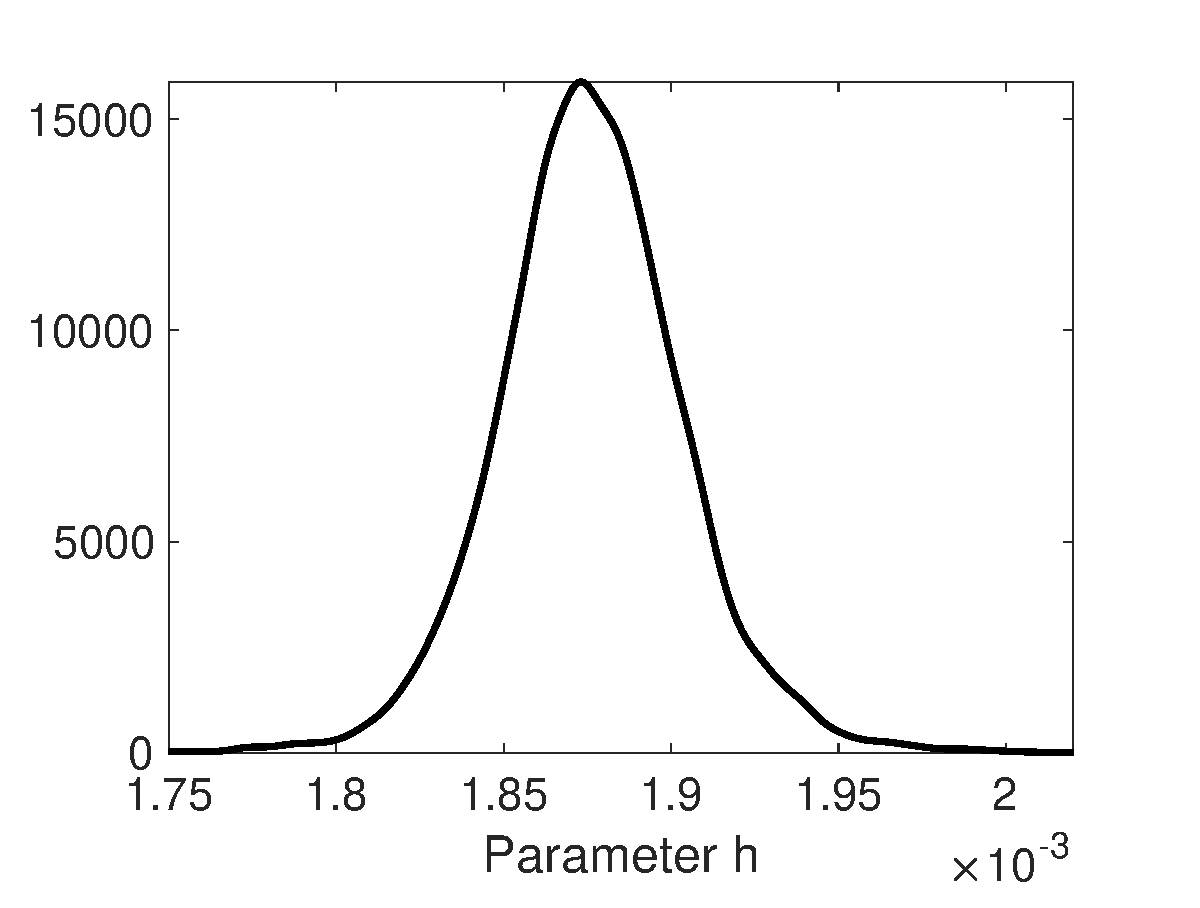
\includegraphics[ width=.5\linewidth]{Figures/2b.eps}}\\
         \subfloat[]{%
      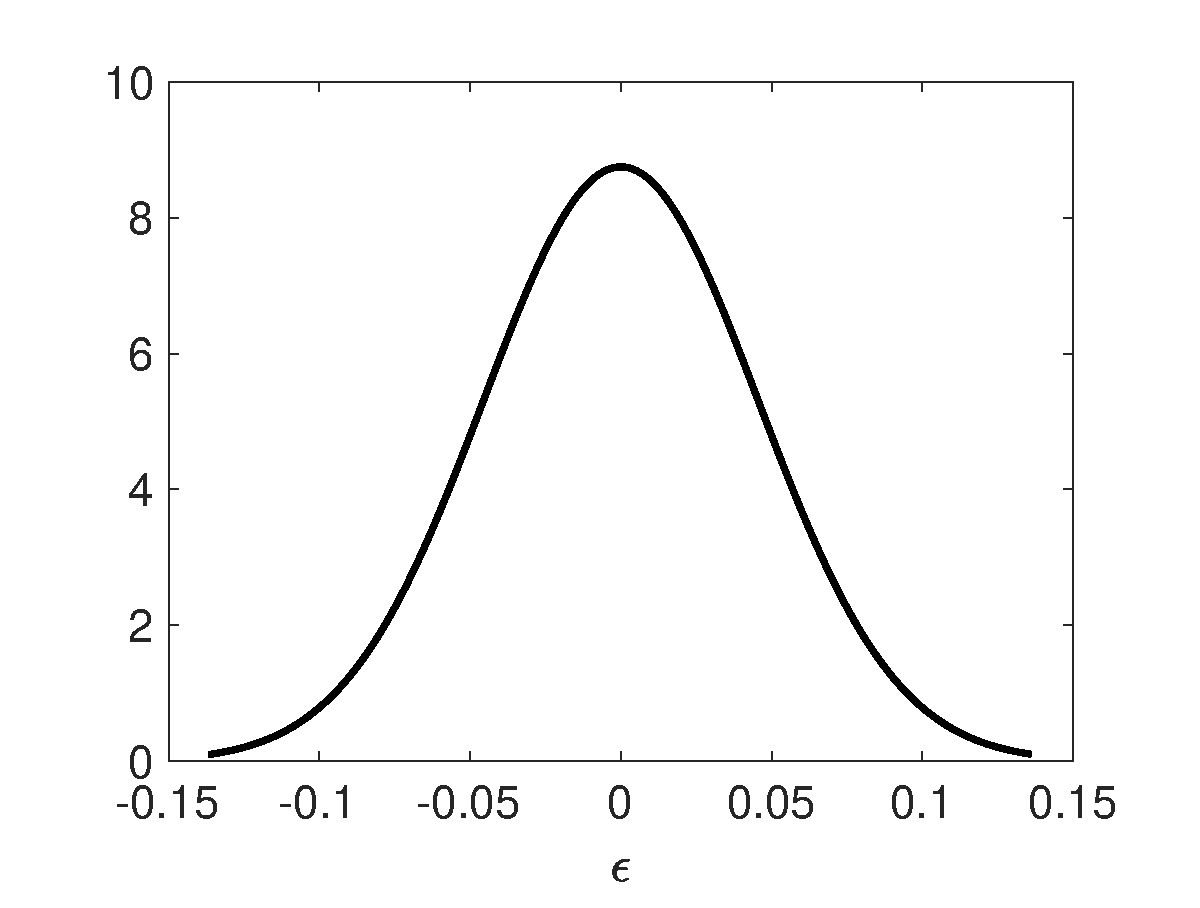
\includegraphics[ width=.5\linewidth]{Figures/2a.eps}}\\
\caption{Densities for (a) $\Phi$; (b) $h$; (c) $\varepsilon$}
\label{fig2}
\end{figure*}
Next, we used the DRAM commands {\bf mcmcpred} and {\bf mcmcpredplot} to construct $95\%$ credible and prediction intervals for the given data in Table \ref{tab2}. From Figure \ref{fig2}, we observed that the error variance and variance of the parameters are small. Hence, when we propagate the model response, the credible and prediction intervals are small. As a result, we obtained the zoomed version of part (a) in Figure \ref{fig3}(b) to demonstrate the difference between credible and non-credible prediction intervals.
\begin{figure*}[!hbt]
   \subfloat[]{%
      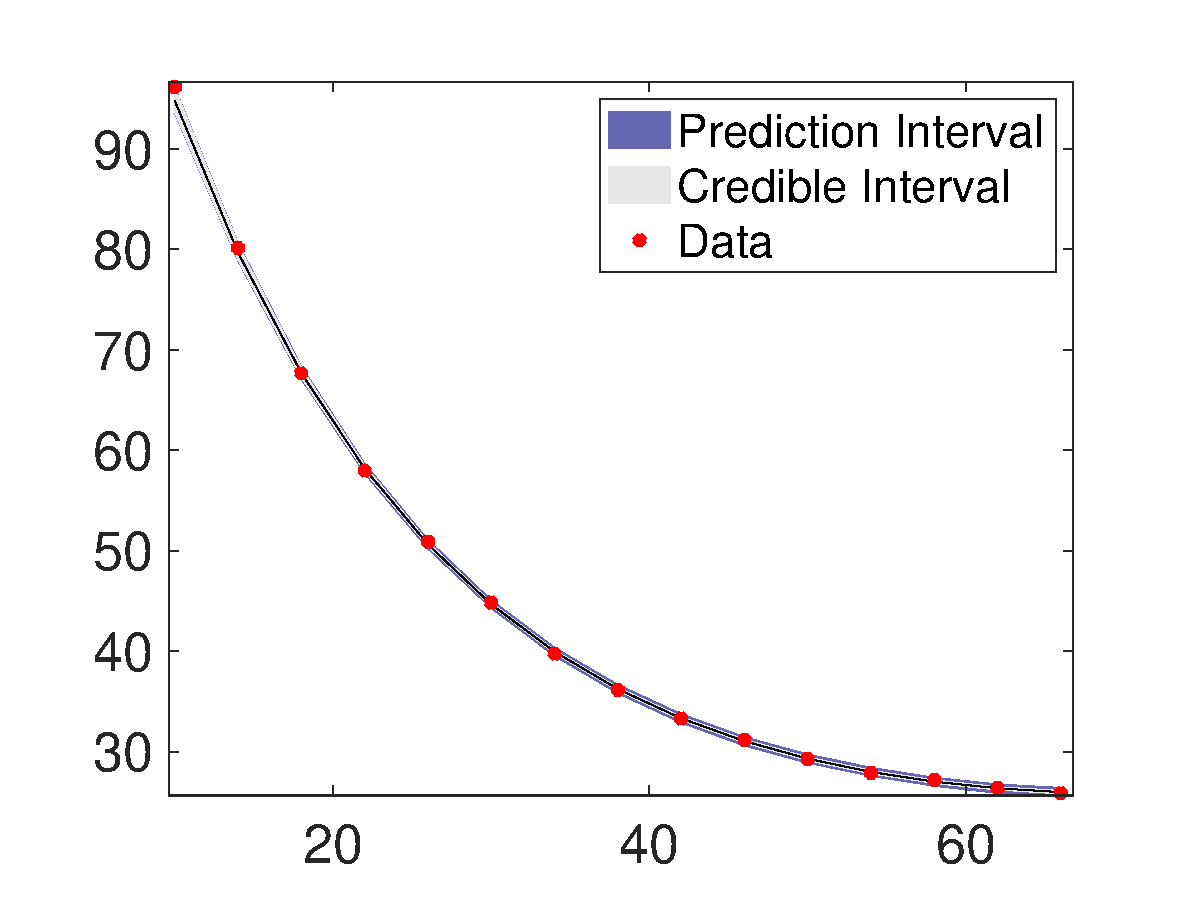
\includegraphics[ width=.5\linewidth]{Figures/2_d.eps}}
   \subfloat[]{%
      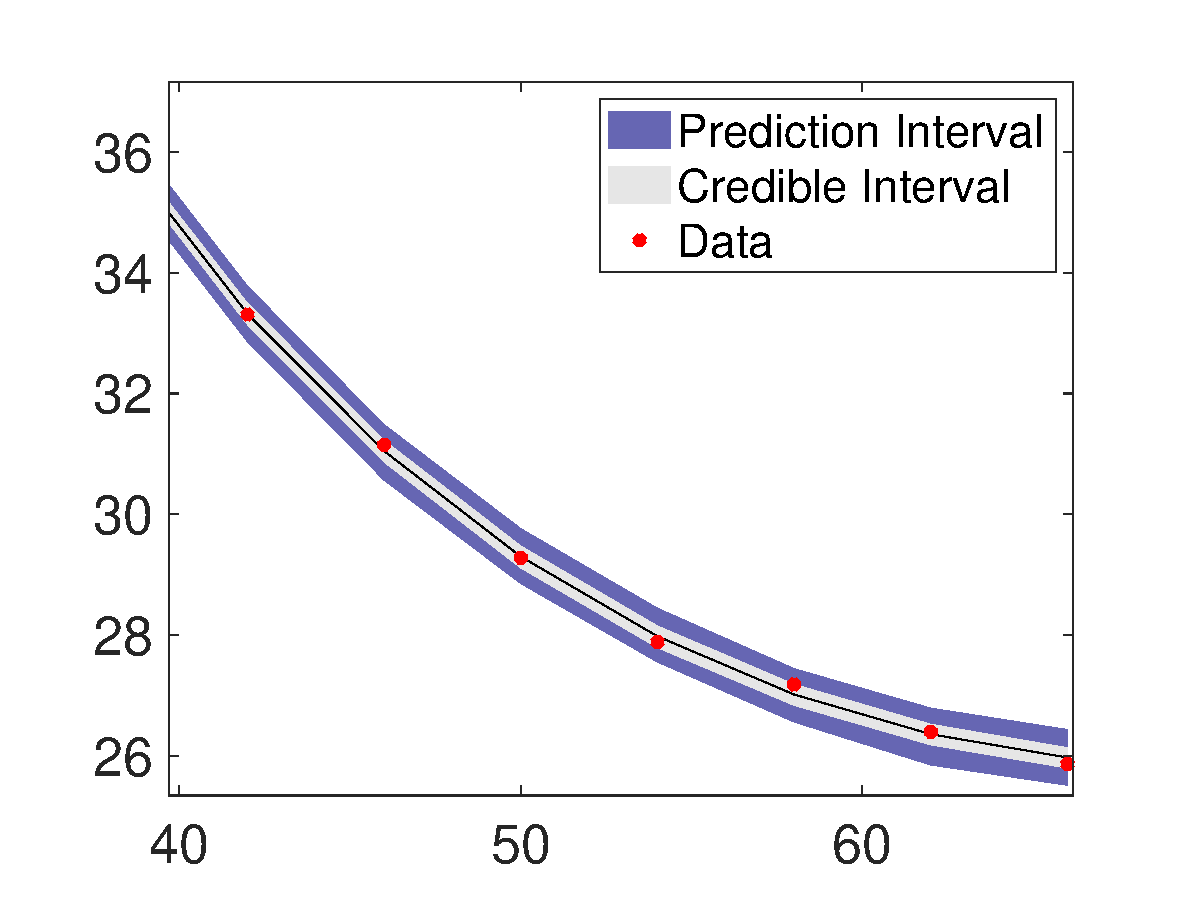
\includegraphics[ width=.5\linewidth]{Figures/2_e.eps}}
\caption{(a) Data, $95\%$ credible and prediction interval using data in Table \ref{tab2}; (b) Reduced x-axis to illustrate the difference of credible and prediction interval.}
\label{fig3}
\end{figure*}

\item Consider the SIR model
 \begin{align*}
    \frac{d\, S}{dt}&=\delta N-\delta S-\gamma  I S,  \qquad \quad  S(0)=900\\
    \frac{d\, I}{dt}&=\gamma  I S-(r+\delta)I, \quad\, \qquad  I(0)=100\\
     \frac{d\, R}{dt}&=rI-\delta R, \qquad  \qquad \qquad \,\,\, R(0)=0
    \end{align*} where $\gamma, r$ and $\delta$ are each in the interval [0, 1].
    \begin{enumerate}
        \item The file {\bf SIR.txt} contains times $t_i$ in the first column and corresponding values $I(t_i)$ in the second, and the parameters $\pmb{\theta} = [\gamma, r,\delta ]$. Employ DRAM to compute parameter chains in the manner investigated in Exercise 12.8. Use the DRAM commands {\bf mcmcpred} and {\bf mcmcpredplot}, to construct $95\%$ credible and prediction intervals for $I(t)$ and plot with the data from {\bf SIR.txt}
        \item Consider the influenza, as detailed in Exercise 11.7(d), you can employ $ \delta= 0$ and the initial values $S(0) = 730$, $I(0) = 3$ and $R(0) = 0$ so that $N = 733$. Employ DRAM to compute parameter chains in the manner investigated in Exercise 12.8(c). Construct $95\%$ credible and prediction intervals for $I(t)$ and plot with the data in Table \ref{tab4}.
\begin{table}[!htb]
\centering
\begin{tabular}{|l|l|l|l|l|l|l|l|l|l|l|l|l|l|l|}
\hline
\multicolumn{1}{|c|}{Day} & 0 & 1 & 2  & 3  & 4   & 5   & 6   & 7   & 8   & 9   & 10 & 11 & 12 & 13 \\ \hline
Confined to Bed           & 3 & 8 & 26 & 76 & 225 & 298 & 258 & 233 & 189 & 128 & 68 & 29 & 14 & 4  \\ \hline
\end{tabular}
\caption{Influenza data}
\label{tab4}
\end{table}   

    \end{enumerate}
    
{\em Solution.} 

\begin{enumerate}
    \item Since we performed Bayesian model calibration using DRAM in the previous project, we skipped that part. It’s worth noting that the chains are converged. Hence, we can use these results to propagate parameter uncertainty for the model response. Then, using the DRAM commands {\bf mcmcpred} and {\bf mcmcpredplot}, we construct $95\%$ credible andprediction intervals for given data in $\mathbf{SIR.txt}$. Figure \ref{fig4}(a) shows the graphs of the credible and prediction intervals.
    \item We used the DRAM algorithm for this problem in Project 3. Here we observed that the chains have all converged. Since we have a converged chain, we obtained the $95\%$ credible intervals using posterior samples. The graph in Figure \ref{fig4} was obtained using the {\bf mcmcpred} and {\bf mcmcpredplot} commands.
\end{enumerate}

\begin{figure*}[!hbt]
   \subfloat[]{%
      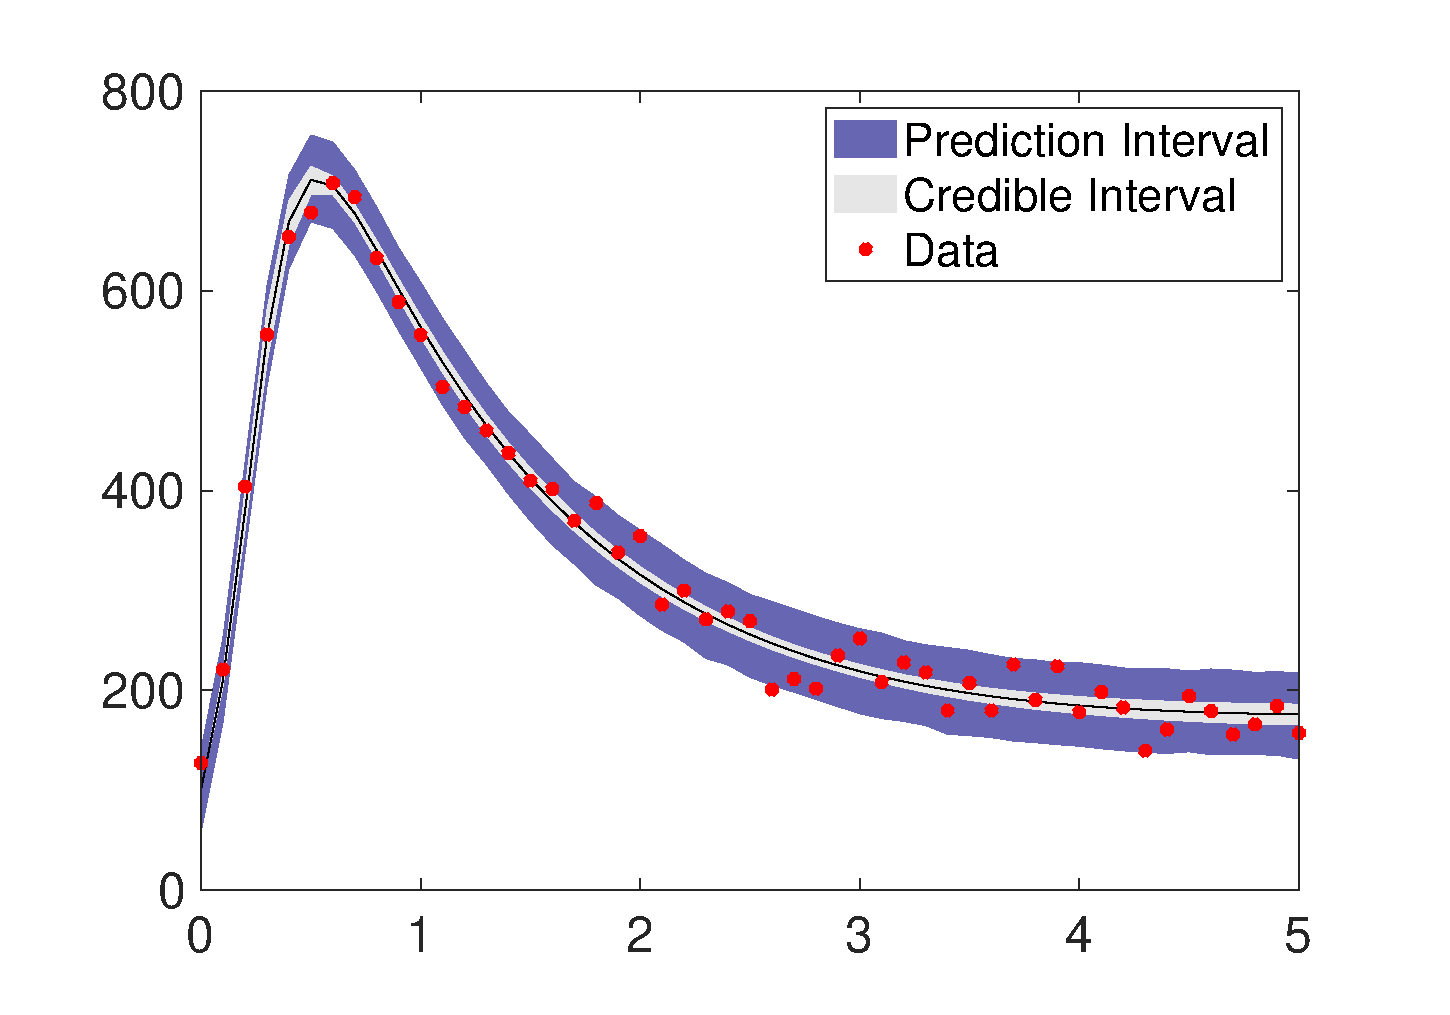
\includegraphics[ width=.54\linewidth]{Figures/3a.eps}}
   \subfloat[]{%
      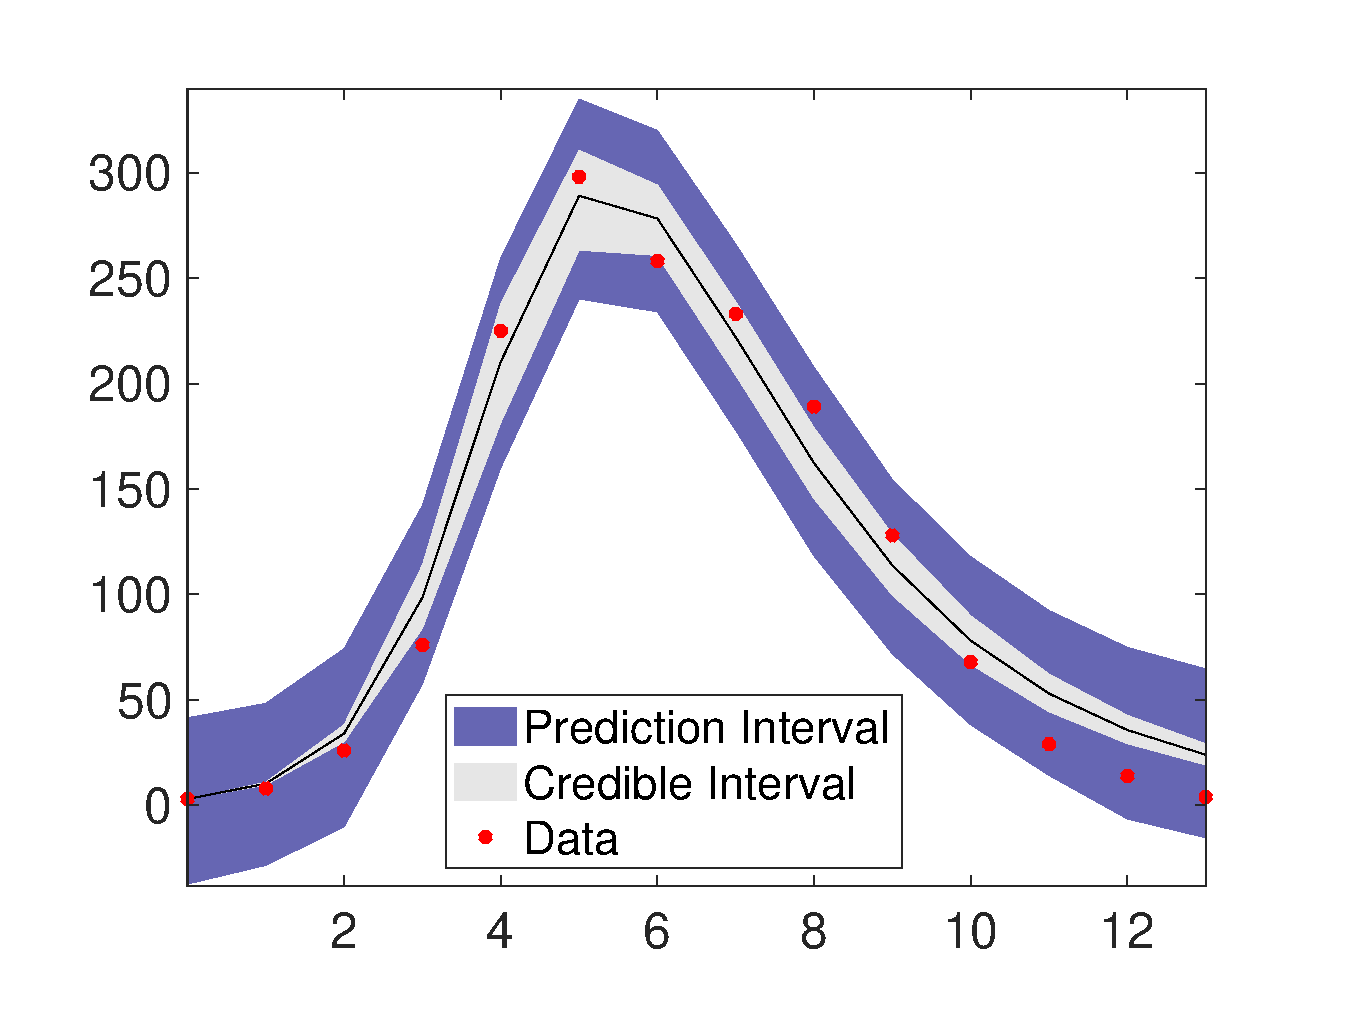
\includegraphics[ width=.5\linewidth]{Figures/3b.eps}}
\caption{Data, $95\%$ credible and prediction interval using (a) data in $\mathbf{SIR.txt}$; (b) Influenza data, Table \ref{tab4}.}
\label{fig4}
\end{figure*}
    \item Consider the SIR model from Exercise 13.5 with parameters $\pmb{\theta} = [\gamma, r,\delta ]$. The file ${\bf SIR.txt}$ contains times $t_i$ and corresponding values $I(t_i)$. Employ the complex-step or sensitivity equation code posted for Example 8.9 to estimate the sensitivity matrix $\mathbf{S}$ having entries $[\mathbf{S}]_{ij} = \frac{ \partial I}{\partial \theta_j}(t_i, \pmb{\bar\theta})$ 
for the nominal parameter values $\pmb{\bar \theta}=  [0.0100; 0.7970; 0.1953]$ estimated in Exercise 11.7. You can employ the estimate $ \sigma^2= 426.8$ from that example. Use the sensitivity matrix to estimate the parameter covariance matrix $\mathbf{V}$ and construct the response and observation matrices
$$\mbox{var}[\pmb{f(\theta)}] = \mathbf{SVS}^\top$$
$$\mbox{var}[\mathbf{Y}] = \mathbf{SVS}^\top + \sigma^2 \mathbf{I}_{n\times n}.$$ Let  $\sigma_{\pmb{f}}(t_i)$ and $\sigma_{\mathbf{Y}}(t_i)$ denote the square roots of the diagonal elements. Plot $I(t_i)$ and the $\pm 2\sigma_{\pmb{f}}(t_i)$ and $\pm 2\sigma_{\mathbf{Y}}(t_i)$ intervals and compare with the $95\%$ credible and prediction intervals computed in Exercise 13.5. What do you conclude about the accuracy of the linearization?

\begin{figure*}[!ht]
\centering
      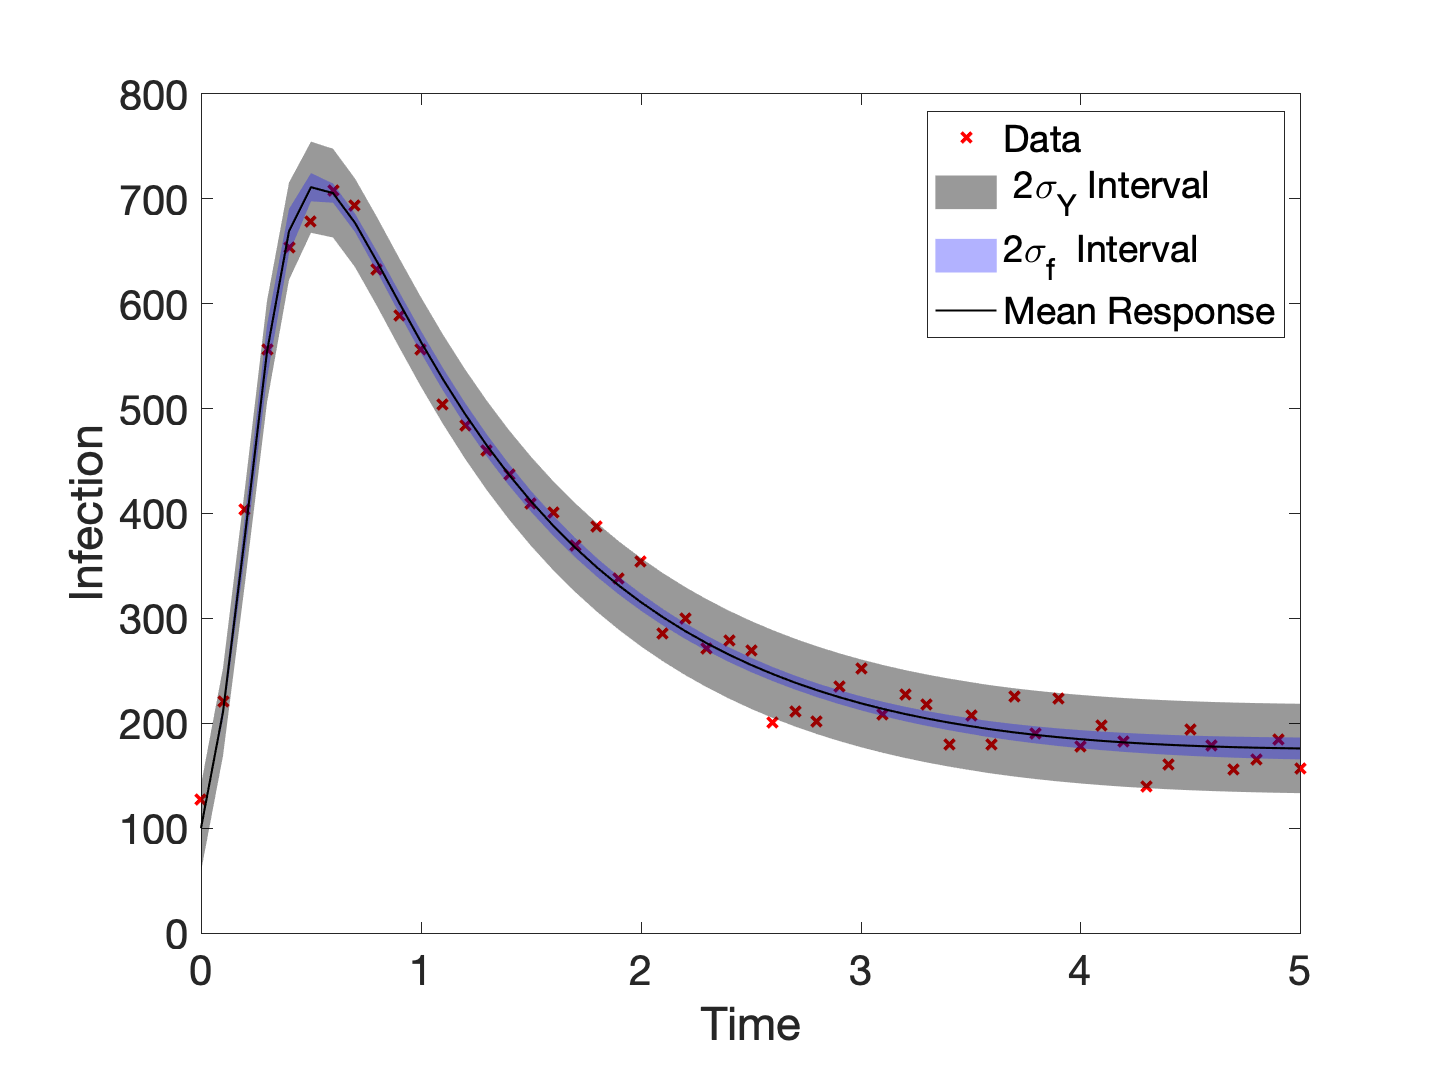
\includegraphics[ width=.75\linewidth]{Figures/4.eps}
\caption{Data, $\pm2\sigma_\mathbf{f}$ and $\pm 2\sigma_\mathbf{Y}$ interval using data in $\mathbf{SIR.txt}$.}
\label{fig5}
\end{figure*}



{\em Solution} 


Using complex step approximation, $$f'(x)\approx\frac{Im(f(x+ih))}{h},$$  and the optimal parameters obtained by frequentist approach we get the sensitivities of the response, $I(t),$ to the each parameter. By utilizing it, we obtained the sensitivity matrix $\mathbf{S}$ having entries $[\mathbf{S}]_{ij} = \frac{ \partial I}{\partial \theta_j}(t_i, \pmb{\bar\theta}).$ Employing  estimated variance and sensitivity matrix we obtained the covariance matrix, $\mathbf{V}.$ Next using sensitivity matrix and  covariance matrix we obtained the response and observation matrices
$$\mbox{var}[\pmb{f(\theta)}] = \mathbf{SVS}^\top$$
$$\mbox{var}[\mathbf{Y}] = \mathbf{SVS}^\top + \sigma^2 \mathbf{I}_{n\times n}$$ where both of them are $51\times 51$ matrices, since we have $n=51$ data points. In this case the mean response would be $I(t_i,\pmb{\bar \theta}),$ the $\pm 2\sigma_{\pmb{f}}(t_i)$ interval is 
$$ \bigg[I(t_i,\pmb{\bar \theta})\pm 2\sqrt{(\mbox{var}[\pmb{f(\theta)}])_{ii}} \bigg]$$  and the $\pm 2\sigma_{\mathbf{Y}}(t_i)$ interval is 
$$ \bigg[I(t_i,\pmb{\bar \theta})\pm 2\sqrt{(\mbox{var}[\mathbf{Y}])_{ii}} \bigg].$$ The intervals are given in Figure \ref{fig5}.  We can observe that this intervals are narrower than Bayesian $95\%$ credible and prediction interval given in Figure \ref{fig4}. But the difference is not big, so we can conclude that accuracy of the linearization is high.

\end{enumerate}





\end{document}

